\documentclass{standalone}
\usepackage{pgfplots}
\pgfplotsset{compat=1.18} % Use the latest version for better compatibility

\begin{document}

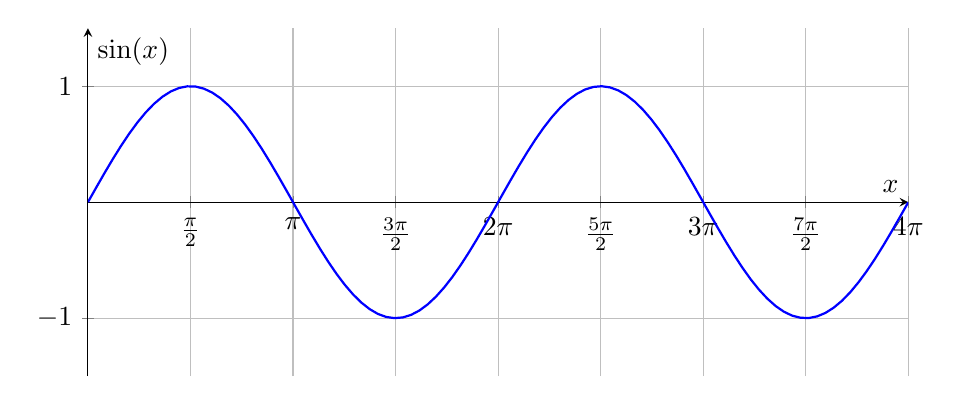
\begin{tikzpicture}
  \begin{axis}[
      domain=0:4*pi, % Domain of the plot
      xmin=0, xmax=4*pi, % X-axis limits
      ymin=-1.5, ymax=1.5, % Y-axis limits
      xtick={0, pi/2, pi, 3*pi/2, 2*pi, 5*pi/2, 3*pi, 7*pi/2, 4*pi}, % Tick marks every pi/2
      xticklabels={
        0,
        $\frac{\pi}{2}$,
        $\pi$,
        $\frac{3\pi}{2}$,
        $2\pi$,
        $\frac{5\pi}{2}$,
        $3\pi$,
        $\frac{7\pi}{2}$,
        $4\pi$
      }, % Labels for tick marks
      ytick={-1, 0, 1}, % Y-axis tick marks
      xlabel={$x$}, % X-axis label
      ylabel={$\sin(x)$}, % Y-axis label
      grid=both, % Add grid lines
      width=12cm, % Width of the plot
      height=6cm, % Height of the plot
      axis lines=middle, % Axis lines in the middle
      samples=100, % Number of samples for smooth curve
    ]
    \addplot[blue, thick] {sin(deg(x))}; % Plot sin(x)
  \end{axis}
\end{tikzpicture}

\end{document}